\usepackage[T1]{fontenc}
\usepackage[utf8]{inputenc}
\usepackage[portuguese]{babel}
\usepackage{graphicx} %permite inserir figuras
\usetheme{Frankfurt}


\begin{frame}
\frametitle{Plano de Desenvolvimento}
\begin{minipage}{.5\linewidth}
\begin{figure}[ht]
\begin{flushleft}
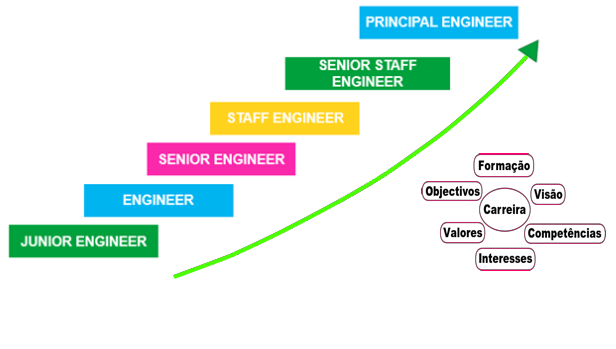
\includegraphics[scale=0.35]{./image/Career_Path/Progressao.png}
\end{flushleft}
\end{figure}
\end{minipage}
\begin{minipage}{.45\linewidth}
\begin{figure}[ht]
	\begin{flushleft}
		
\includegraphics[scale=0.25]{./image/Career_Path/Old_Age.jpeg}
	\end{flushleft}\vfill
	\begin{flushright}
		
\includegraphics[scale=0.1]{./image/Career_Path/Burial.jpeg}
	\end{flushright}
\end{figure}
\end{minipage}
\vfill
\hfill {\tiny Sérgio Santos}
\end{frame}



\tableofcontents
%\appendix
\pagestyle{plain} %plain headings empty
%\setcounter{chapter}{0}
%\numberwithin{page}{section}
\renewcommand{\abstractname}{Executive Summary}
\setlength{\parindent}{0in}
%\renewcommand{\columnsep}{1cm}.
%%%%%%%%%%%%%%%%%%%%%%%%%%%%%%%%%%%%%%%%%%%%%%%%%%%%%%%%%%%%%%%%%%%%%%%%%%%%%%%%%%%%%%%%%%%%%%%%%%%
\newpage
\begin{abstract}
This document presents the basic concepts of typesetting in a
form usable by non-specialists. It is aimed at those who find
themselves (willingly or unwillingly) asked to undertake work
previously sent out to a professional printer, and who are
concerned that the quality of work (and thus their corporate
image) does not suffer unduly.
The topics cover layout, the need for accuracy, the choice of
typeface, arrangement of the document, adherence to
specifications, and the production process. No foreknowledge
of printing or publishing is needed, but an eye for detail,
a feeling for æsthetics, and some fluency with a computer is
expected.
\end{abstract}


\begin{raggedleft}
These modes also exist as environments called raggedright and
raggedleft which is more convenient when applying this formatting
to a whole paragraph or more, like this one.
\end{raggedleft}


\[\bar nˆ*_j(s)=\frac{\left\{s\sumˆk_{i=1}n_i(0)pˆ*
_{i,k+1}(s)+Mˆ*(s)\right\}\sumˆk_{i=1}p_{0i}pˆ*{ij}
(s)}{1-s\sumˆk_{i=1}p_{0i}pˆ*_{i,k+1}(s)}+\sumˆk
_{i=1}n_i(0)pˆ*_{ij}(s)[j=1,2,\dots,k].\]


\begin{itemize}
\item Itemized lists usually have a bullet;
\item Long items use ‘hanging indentation’, whereby the
text is wrapped with a margin which brings it clear of
the bullet used in the first line of each item;
\item The bullet can be changed for any other symbol, for
example from the \textsf{bbding} or \textsf{pifont} package.
\end{itemize}

\begin{enumerate}
\item Enumerated lists use numbering on each item;
\item Long items use ‘hanging indentation’ just the same
as for itemized lists;
\item The numbering system can be changed for any level.
\end{enumerate}

\begin{description}
\item[Identification:] description lists require a topic
for each item given in square brackets;
\item[Hanging indentation:] Long items use this in the
same way as all other lists;
\item[Reformatting:] Long topics can be reprogrammed to
fold onto multiple lines.
\end{description}

\textbf{\itshape Inline lists}, which are sequential in
nature but are \begin{inparaenum}[\itshape a\upshape)]
\item formatted within their paragraph
\item usually labelled with letters\end{inparaenum},
like this example. The items are Boolean, with the final
item prefixed by ‘and’ or ‘or’.

\newpage

\begin{table}
\caption{Project expenditure to year-end 2001}
\label{ye2001exp}
...
\end{table}

\begin{table}
\caption{Project expenditure to year-end 2001}
\label{ye2001exp}
\begin{center}
\begin{tabular}{clr}
&Item&Amount\\
\hline
a)&Salaries (2 research assistants)&28,000\\
&Conference fees and travel expenses&14,228\\
&Computer equipment (5 workstations)&17,493\\
&Software&3,562\\
b)&Rent, light, heat, power, etc&1,500\\\cline{3-3}
&Total&64,783
\end{tabular}
\par\medskip\footnotesize
The Institute also contributes to (a) and (b).
\end{center}
\end{table}


%\begin{figure}
%\caption{Total variable overhead variance (after
%\citeauthor[p.191]{bull}}
%\label{workeff}
%\begin{center}
%\fbox{\includegraphics[width=.5\columnwidth]{diagram}}
%\end{center}
%\end{figure}


\parbox{1in}{Please make sure you send in your completed
forms by January 1st next year, or the penalty
clause 2(a) will apply}


\begin{minipage}{3in}
Please make sure you send in your completed forms by January
1st next year, or the penalty clause 2(a) will apply.
\begin{itemize}
\item Incomplete forms will be returned to you unprocessed.
\item Forms must be accompanied by the correct fee.
\item There is no appeal. The adjudicators’ decision is final.
\end{itemize}
\end{minipage}

\setlength{\fboxsep}{1em}
\setlength{\fboxrule}{2pt}

\fbox{\begin{tabular}{p{1in}}
Multiline text in a box typeset using \textsf{tabular}
\end{tabular}}
\vspace{20cm}
\fbox{\begin{minipage}{3in}
This multiline text is more flexible than a tabular
setting:
\begin{itemize}
\item it can contain any type of normal \LaTeX{}
typesetting;
\item it can be any specified width;
\item it can even have its own footnotes\footnote{Like
this}.
\end{itemize}
\end{minipage}}

\begin{quote}
Do, Ronny, Do. \textit{Nancy Reagan}
Da Do Ron Ron \textit{The Crystals}
\end{quote}


\begin{quotation}\small
At the turn of the century William Davy, a Devonshire
parson, finding errors in the first edition of his
%\citetitle{davy}, asked for a new edition to be
printed. His publisher refused and Davy purchased a
press, type, and paper. He harnessed his gardener to
the press and apprenticed his housemaid to the
typesetting. After twelve years’ work, a new
edition of fourteen sets of twenty-six volumes was
issued---which surely indicates that, when typomania
is coupled with religious fervour, anything up to a
%miracle may be achieved.\citequote[p.76]{ryder}
\end{quotation}


\begin{multicols}{3}
...
\end{multicols}



\begin{minipage}[t]{.49\textwidth}
\flushleft
Some long testing text to illustrate the alignment problem.
\end{minipage}
%
\hfill
%
\noindent
\begin{minipage}[t]{.49\textwidth}
\flushright
\begin{tabular}{r l}
\textbf{Some Long Label} & Bar \\
\textbf{Another Long Label} & Foo Bar Baz \\
\end{tabular}
\end{minipage}













\newpage
%%%%%%%%%%%%%%%%%%%%%%%%%%%%%%%%%%%%%%%%%%%%%%%%%%%%%%%%%%%%%%%%%%%%%%%%%%%%%%%%%%%%%%%%%%%%%%%%%%%
%Figuras Bibliografia Index
\listoffigures
\cite{*}
\bibliography{./bibliography/Bibliography}
%\printindex
\newpage
\footnote{Apontamento}
\end{document}
%%%%%%%%%%%%%%%%%%%%%%%%%%%%%%%%%%%%%%%%%%%%%%%%%%%%%%%%%%%%%%%%%%%%%%%%%%%%%%%%%%%%%%%%%%%%%%%%%%%
